% !TeX root = ../dokumentation.tex

\addchap{\langanhang}
\renewcommand{\thefigure}{A\arabic{figure}}

\setcounter{figure}{0}

\begin{lstlisting}[label=schemaCol, caption={Schema COLUMN Store}]
DROP TABLE  customer;

CREATE COLUMN TABLE  customer (
	C_CUSTOMERKEY INTEGER,
	C_Name varchar(25),
	C_Address varchar(25),
	C_City varchar(10),
	C_Nation varchar(15),
	C_Region varchar(12),
	C_Phone varchar(15),
	C_MktSegment varchar(10),
	PRIMARY KEY ("C_CUSTOMERKEY")
);

DROP TABLE  part;

CREATE COLUMN TABLE  part
(
	P_PartKey integer,
	P_Name varchar(25),
	P_MFGR varchar(10),
	P_Category varchar(10),
	P_Brand varchar(15),
	P_Colour varchar(15),
	P_Type varchar(25),
	P_Size tinyint,
	P_Container char(10),
	PRIMARY KEY (P_PartKey)
);



DROP TABLE  supplier;

CREATE COLUMN TABLE  supplier (
	S_SuppKey integer,
	S_Name char(25),
	S_Address varchar(25),
	S_City char(10),
	S_Nation char(15),
	S_Region char(12),
	S_Phone char(15),
	PRIMARY KEY(S_SuppKey)
);



DROP TABLE  dim_date;

CREATE COLUMN TABLE  dim_date
(
	D_DateKey integer,
	D_Date char(18),
	D_DayOfWeek char(9),
	D_Month char(9),
	D_Year smallint,
	D_YearMonthNum integer,
	D_YearMonth char(7),
	D_DayNumInWeek tinyint,
	D_DayNumInMonth tinyint,
	D_DayNumInYear smallint,
	D_MonthNumInYear tinyint,
	D_WeekNumInYear tinyint,
	D_SellingSeason char(12),
	D_LastDayInWeekFl tinyint,
	D_LastDayInMonthFl tinyint,
	D_HolidayFl tinyint,
	D_WeekDayFl tinyint,
	PRIMARY KEY(D_DateKey)
);

DROP TABLE lineorder;

CREATE COLUMN TABLE  lineorder
(
	LO_OrderKey bigint not null,
	LO_LineNumber tinyint not null,
	LO_CustKey int not null,
	LO_PartKey int not null,
	LO_SuppKey int not null,
	LO_OrderDateKey int not null,
	LO_OrderPriority varchar(15),
	LO_ShipPriority char(1),
	LO_Quantity tinyint,
	LO_ExtendedPrice decimal,
	LO_OrdTotalPrice decimal,
	LO_Discount decimal,
	LO_Revenue decimal,
	LO_SupplyCost decimal,
	LO_Tax tinyint,
	LO_CommitDateKey integer not null,
	LO_ShipMode varchar(10)
);
\end{lstlisting}

\begin{lstlisting}[label=schemaRow, caption={Schema ROW Store}]
DROP TABLE  customer;

CREATE ROW TABLE  customer (
	C_CUSTOMERKEY INTEGER,
	C_Name varchar(25),
	C_Address varchar(25),
	C_City varchar(10),
	C_Nation varchar(15),
	C_Region varchar(12),
	C_Phone varchar(15),
	C_MktSegment varchar(10),
	PRIMARY KEY ("C_CUSTOMERKEY")
);

DROP TABLE  part;

CREATE ROW TABLE  part
(
	P_PartKey integer,
	P_Name varchar(25),
	P_MFGR varchar(10),
	P_Category varchar(10),
	P_Brand varchar(15),
	P_Colour varchar(15),
	P_Type varchar(25),
	P_Size tinyint,
	P_Container char(10),
	PRIMARY KEY (P_PartKey)
);



DROP TABLE  supplier;

CREATE ROW TABLE  supplier (
	S_SuppKey integer,
	S_Name char(25),
	S_Address varchar(25),
	S_City char(10),
	S_Nation char(15),
	S_Region char(12),
	S_Phone char(15),
	PRIMARY KEY(S_SuppKey)
);



DROP TABLE  dim_date;

CREATE ROW TABLE  dim_date
(
	D_DateKey integer,
	D_Date char(18),
	D_DayOfWeek char(9),
	D_Month char(9),
	D_Year smallint,
	D_YearMonthNum integer,
	D_YearMonth char(7),
	D_DayNumInWeek tinyint,
	D_DayNumInMonth tinyint,
	D_DayNumInYear smallint,
	D_MonthNumInYear tinyint,
	D_WeekNumInYear tinyint,
	D_SellingSeason char(12),
	D_LastDayInWeekFl tinyint,
	D_LastDayInMonthFl tinyint,
	D_HolidayFl tinyint,
	D_WeekDayFl tinyint,
	PRIMARY KEY(D_DateKey)
);

DROP TABLE lineorder;

CREATE ROW TABLE  lineorder
(
	LO_OrderKey bigint not null,
	LO_LineNumber tinyint not null,
	LO_CustKey int not null,
	LO_PartKey int not null,
	LO_SuppKey int not null,
	LO_OrderDateKey int not null,
	LO_OrderPriority varchar(15),
	LO_ShipPriority char(1),
	LO_Quantity tinyint,
	LO_ExtendedPrice decimal,
	LO_OrdTotalPrice decimal,
	LO_Discount decimal,
	LO_Revenue decimal,
	LO_SupplyCost decimal,
	LO_Tax tinyint,
	LO_CommitDateKey integer not null,
	LO_ShipMode varchar(10)
);
\end{lstlisting}

\begin{lstlisting}[label=indizes, caption={Indizes hinzufügen}]
CREATE INDEX idx_c_name ON customer(C_Name);
CREATE INDEX idx_c_city ON customer(C_City);
CREATE INDEX idx_c_region ON customer(C_Region);
CREATE INDEX idx_c_phone ON customer(C_Phone);
CREATE INDEX idx_c_mktsegment ON customer(C_MktSegment);

CREATE INDEX idx_p_name ON part(P_Name);
CREATE INDEX idx_p_mfgr ON part(P_MFGR);
CREATE INDEX idx_p_category ON part(P_Category);
CREATE INDEX idx_p_brand ON part(P_Brand);

CREATE INDEX idx_s_city ON supplier(S_City);
CREATE INDEX idx_s_name ON supplier(S_Name);
CREATE INDEX idx_s_phone ON supplier(S_Phone);

CREATE INDEX idx_lo_orderkey_lo_linenumber ON lineorder(LO_OrderKey, LO_LineNumber);
CREATE INDEX idx_lo_custkey ON lineorder(LO_CustKey);
CREATE INDEX idx_lo_suppkey ON lineorder(LO_SuppKey);
CREATE INDEX idx_lo_partkey ON lineorder(LO_PartKey);
CREATE INDEX idx_lo_orderdatekey ON lineorder(LO_OrderDateKey);
CREATE INDEX idx_lo_commitdatekey ON lineorder(LO_CommitDateKey);
\end{lstlisting}




\begin{lstlisting}[label=importSQL, caption={import.sql}]
IMPORT FROM CSV FILE '/usr/sap/HXE/HDB90/work/date.tbl' INTO "SYSTEM"."DIM_DATE" 
WITH
record delimited by '\n' 
field delimited by '|';

IMPORT FROM CSV FILE '/usr/sap/HXE/HDB90/work/customer.tbl' INTO "SYSTEM"."CUSTOMER" 
WITH
record delimited by '\n' 
field delimited by '|';

IMPORT FROM CSV FILE '/usr/sap/HXE/HDB90/work/lineorder.tbl' INTO "SYSTEM"."LINEORDER" 
WITH
batch 10000
record delimited by '\n' 
field delimited by '|';

IMPORT FROM CSV FILE '/usr/sap/HXE/HDB90/work/part.tbl' INTO "SYSTEM"."PART" 
WITH
record delimited by '\n' 
field delimited by '|';

IMPORT FROM CSV FILE '/usr/sap/HXE/HDB90/work/supplier.tbl' INTO "SYSTEM"."SUPPLIER" 
WITH
record delimited by '\n' 
field delimited by '|';
\end{lstlisting}


\begin{figure}[H]
	\centering
	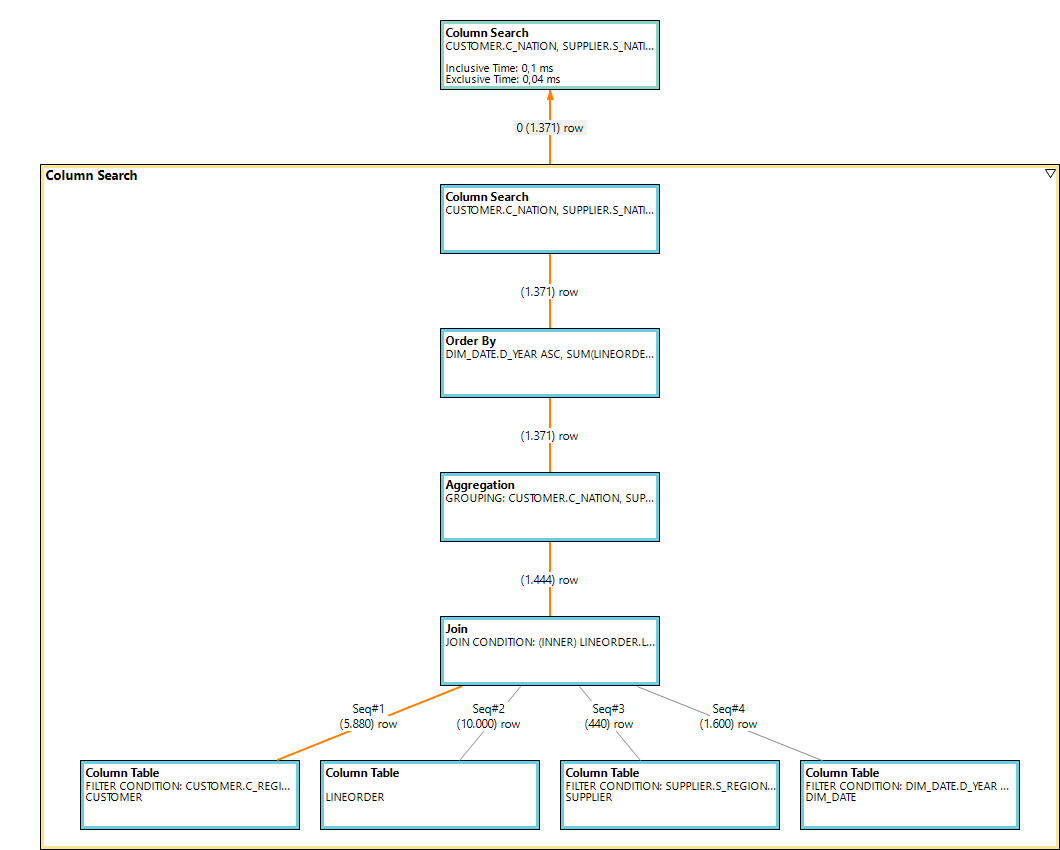
\includegraphics[width=0.7\textwidth]{images/q3-1-col-exec.png}
	\caption{Q3.1 Execution Plan - Comlumn Store}\label{auswertung:q3.1:col}
\end{figure}
\begin{figure}[H]
	\centering
	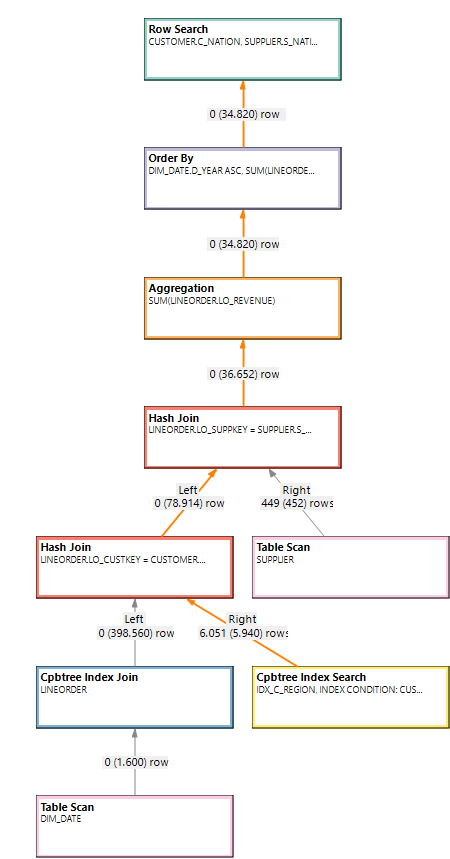
\includegraphics[width=0.7\textwidth]{images/q3-1-row-exec.png}
	\caption{Q3.1 Execution Plan - Row Store}\label{auswertung:q3.1:row}
\end{figure}
\begin{figure}[H]
	\centering
	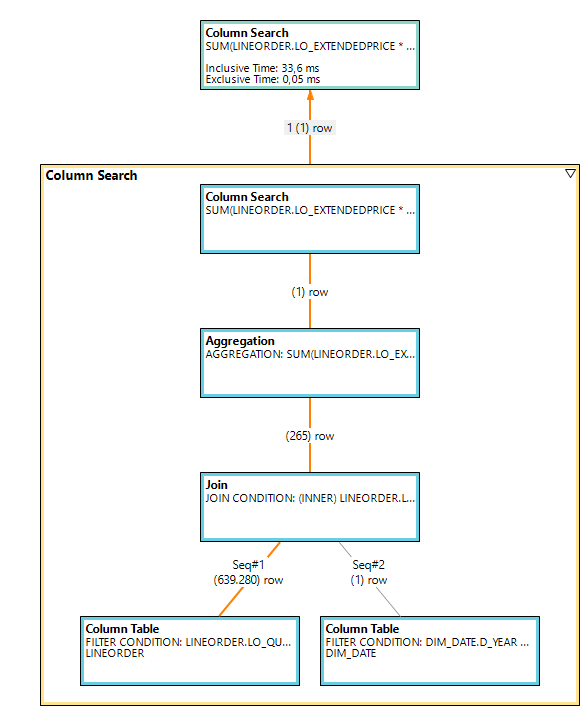
\includegraphics[width=0.7\textwidth]{images/q1-1-col-exec.png}
	\caption{Q1.1 Execution Plan - Column Store}\label{exec:q1.1-col}
\end{figure}
\begin{figure}[H]
	\centering
	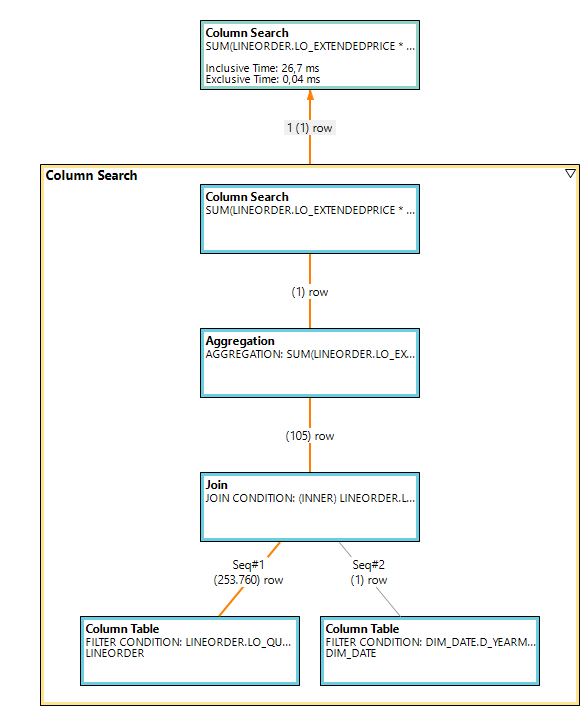
\includegraphics[width=0.7\textwidth]{images/q1-2-col-exec.png}
	\caption{Q1.2 Execution Plan - Column Store}\label{exec:q1.2-col}
\end{figure}
\begin{figure}[H]
	\centering
	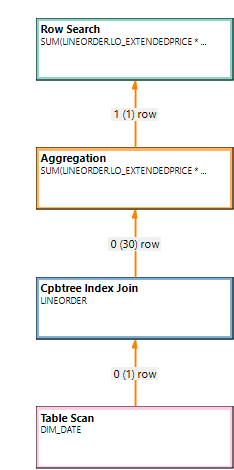
\includegraphics[width=0.7\textwidth]{images/q1-1-row-exec.png}
	\caption{Q1.1 Execution Plan - Row Store}\label{exec:q1.1-row}
\end{figure}
\begin{figure}[H]
	\centering
	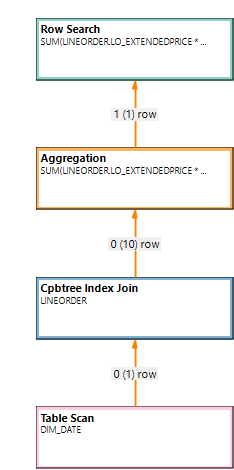
\includegraphics[width=0.7\textwidth]{images/q1-2-row-exec.png}
	\caption{Q1.2 Execution Plan - Row Store}\label{exec:q1.2-row}
\end{figure}


\begin{figure}[H]
	\centering
	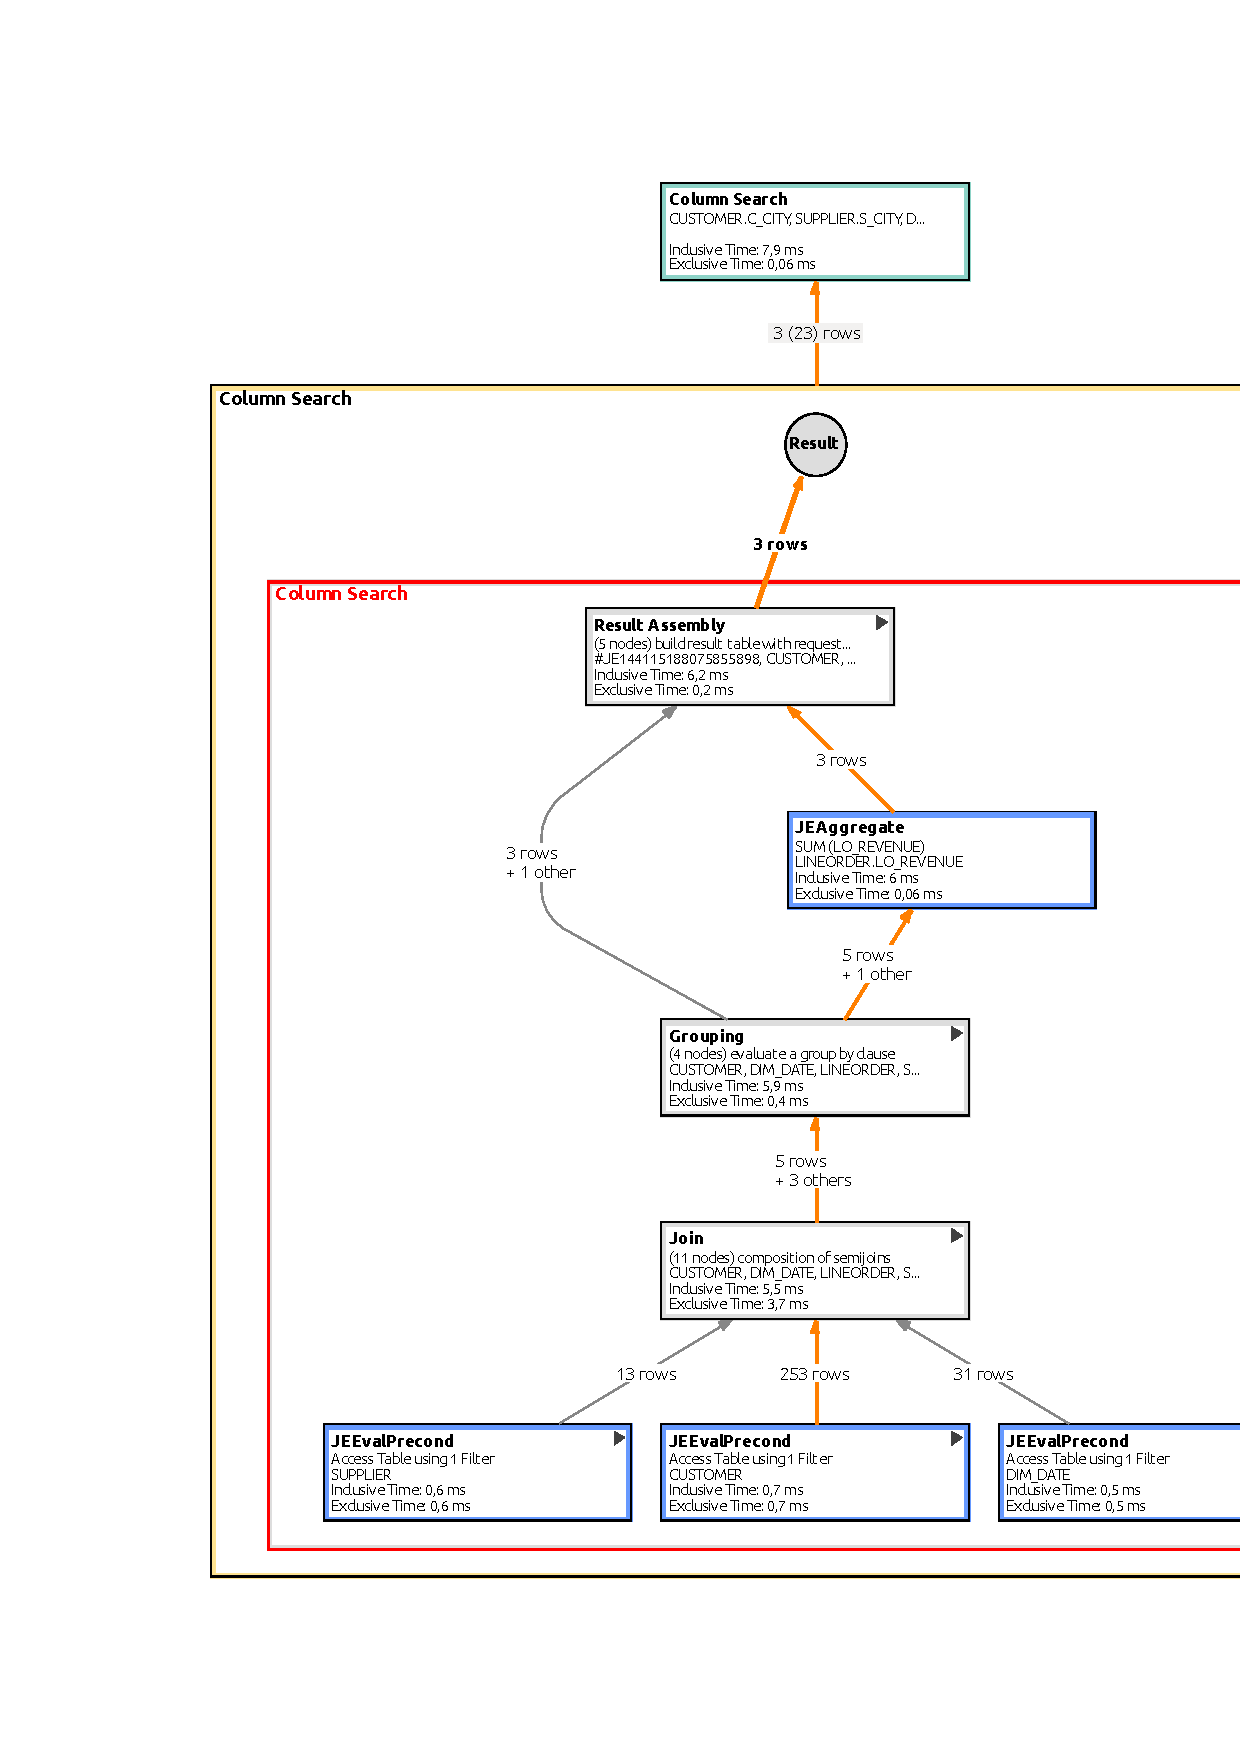
\includegraphics[width=\textwidth]{images/col_q34_index.pdf}
	\caption{Q3.4 Execution Plan - Column Store mit Indizes}\label{exec:q34-col-index}
\end{figure}

\begin{figure}[H]
	\centering
	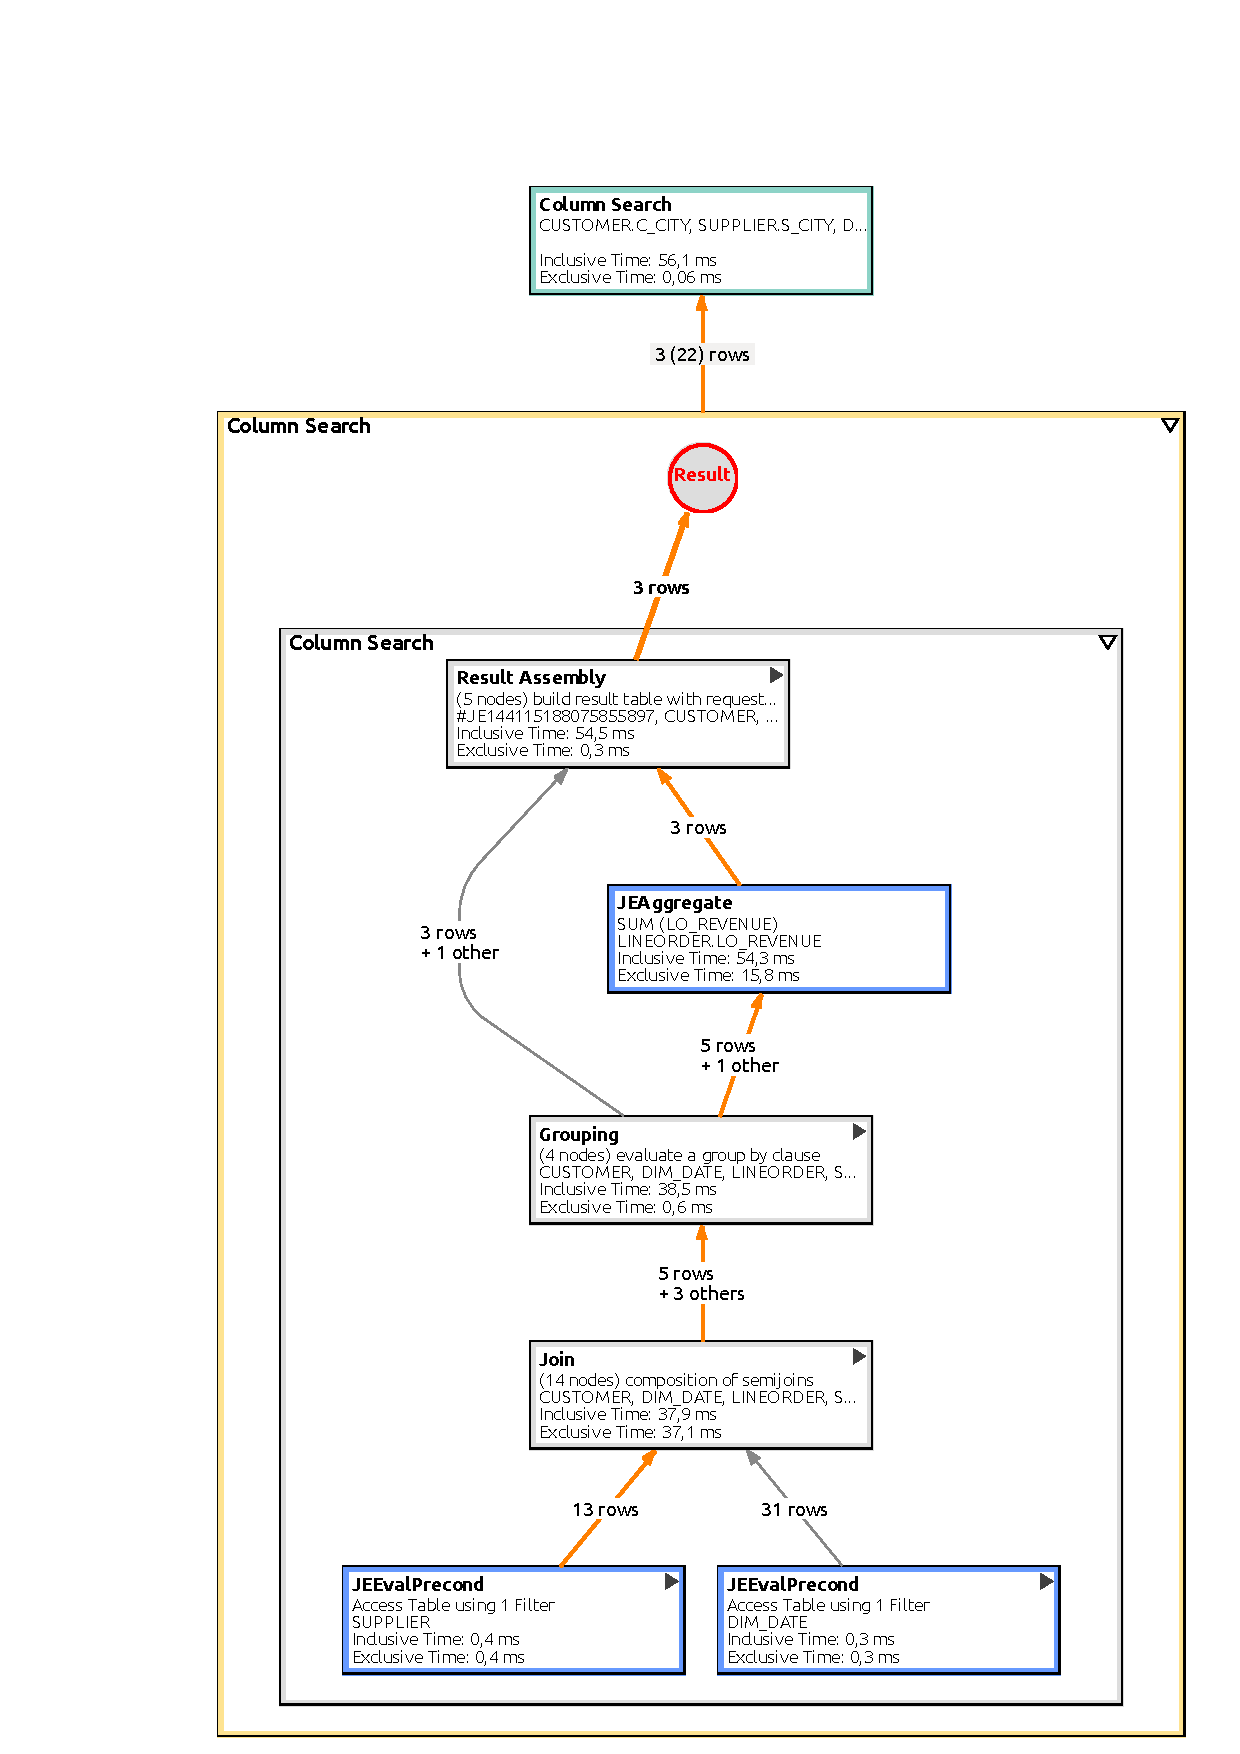
\includegraphics[width=\textwidth]{images/col_q34_no.pdf}
	\caption{Q3.4 Execution Plan - Column Store ohne Indizes}\label{exec:q3.4-col-no}
\end{figure}

\begin{landscape}
	\begin{figure}[H]
		\centering
		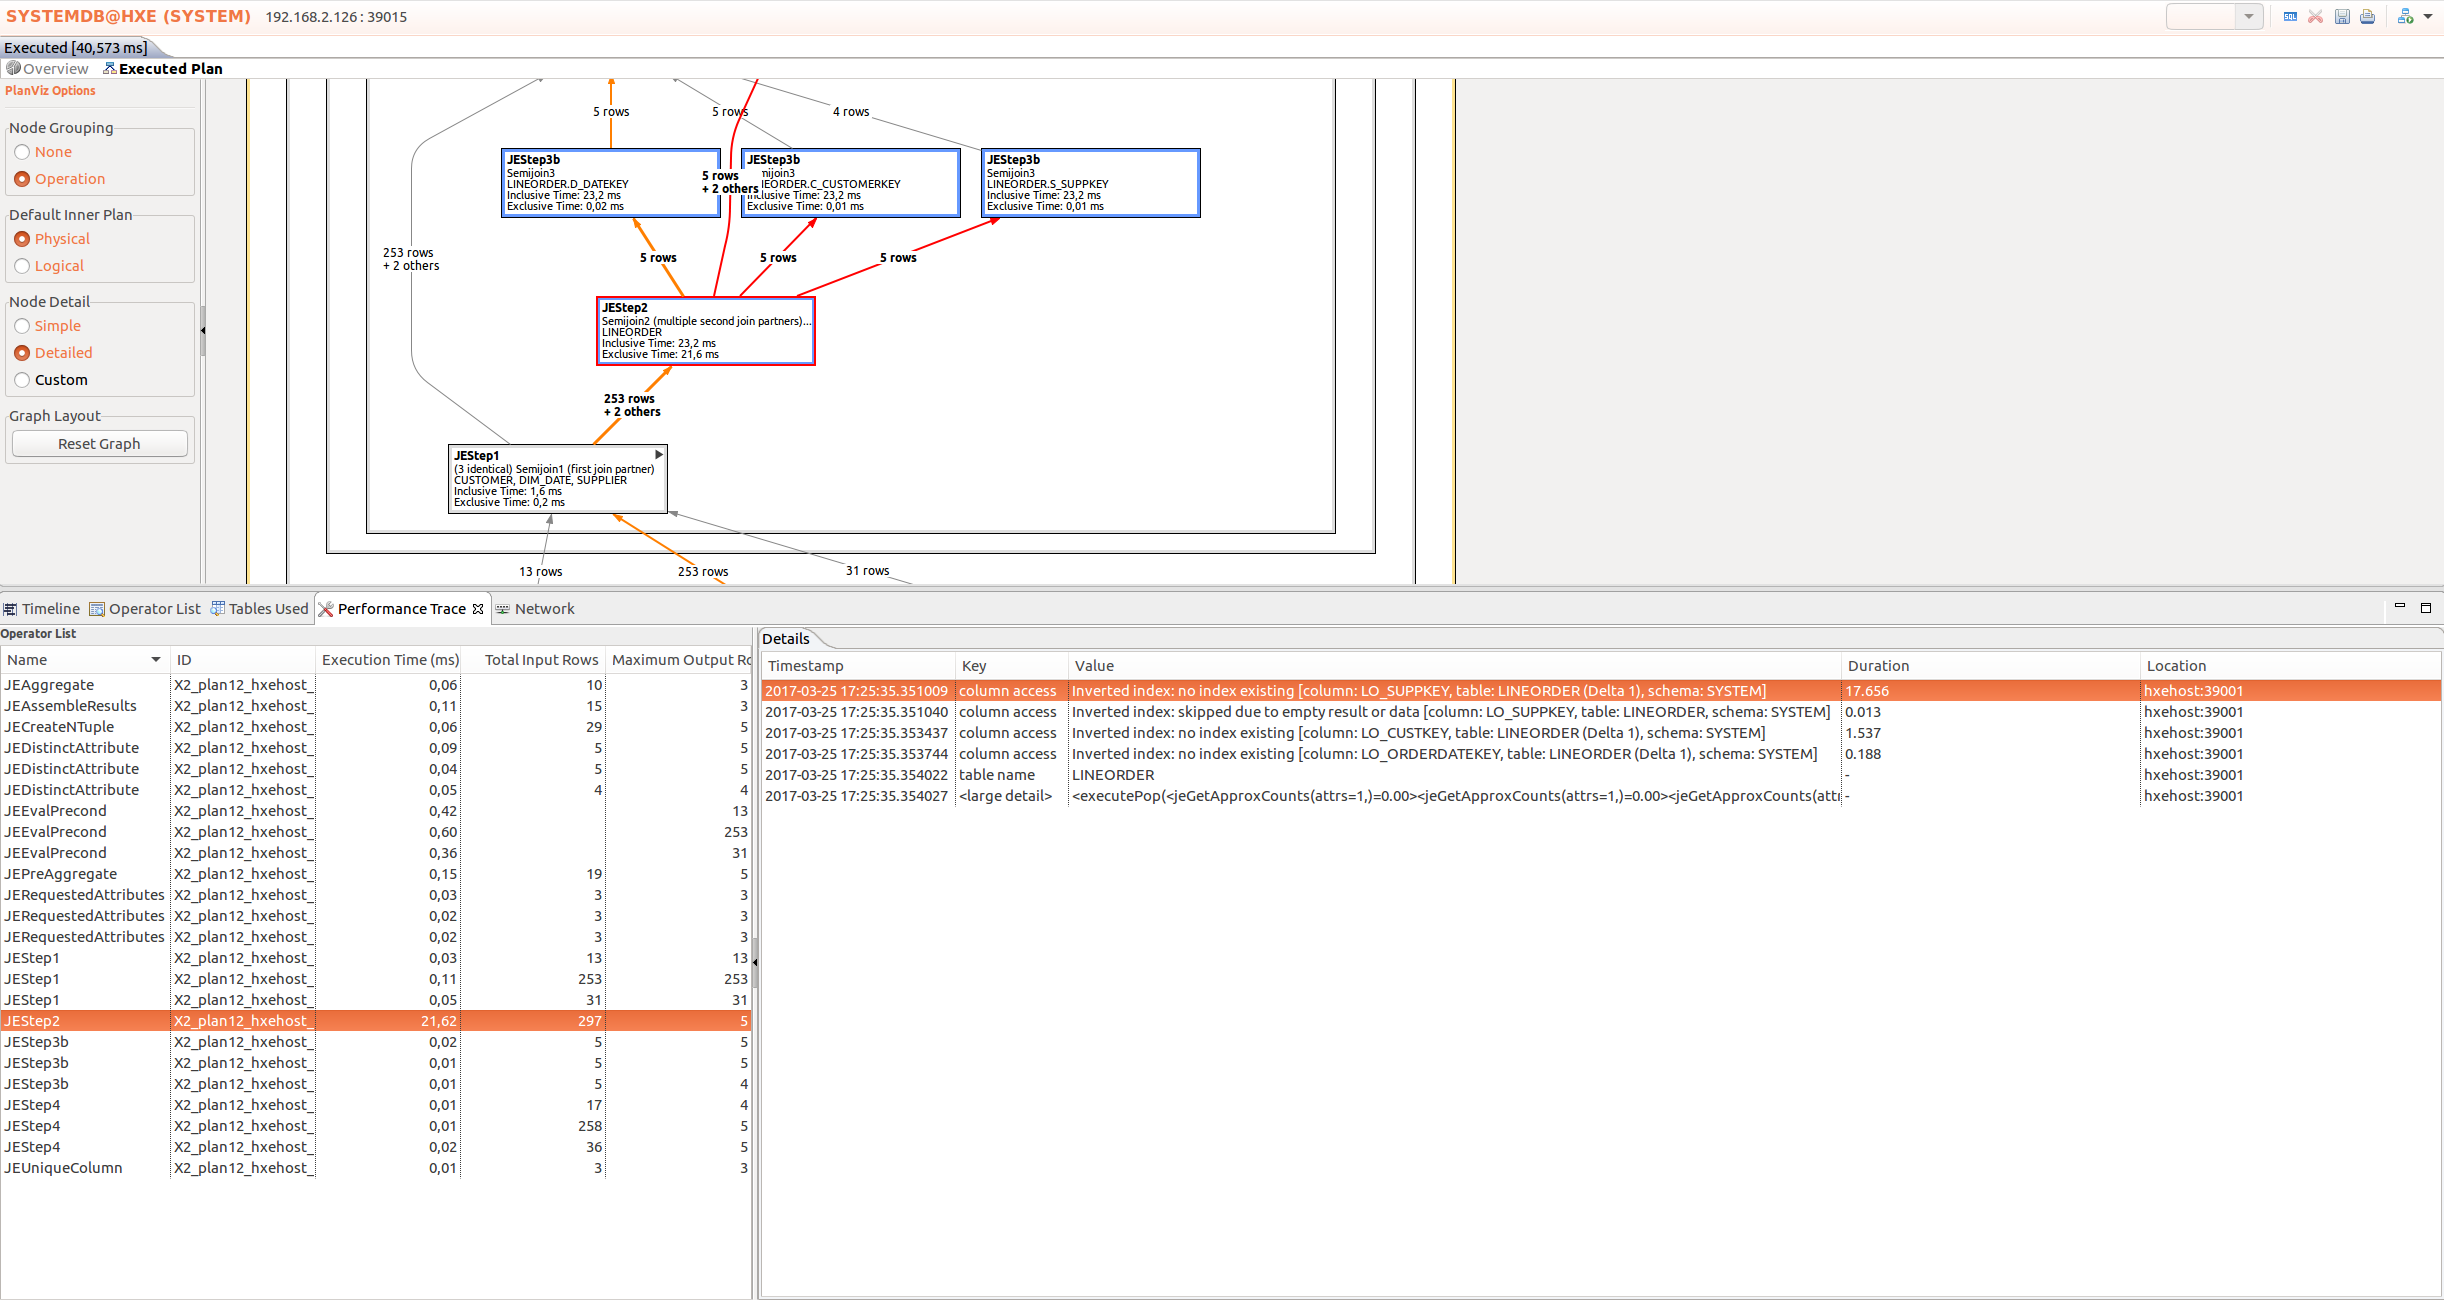
\includegraphics[scale=0.28]{images/execCol.png}
		\caption{Execution Plan: Q3.4}\label{execution-plan:before-index}
	\end{figure}
\end{landscape}
\begin{landscape}
	\begin{figure}[H]
		\centering
		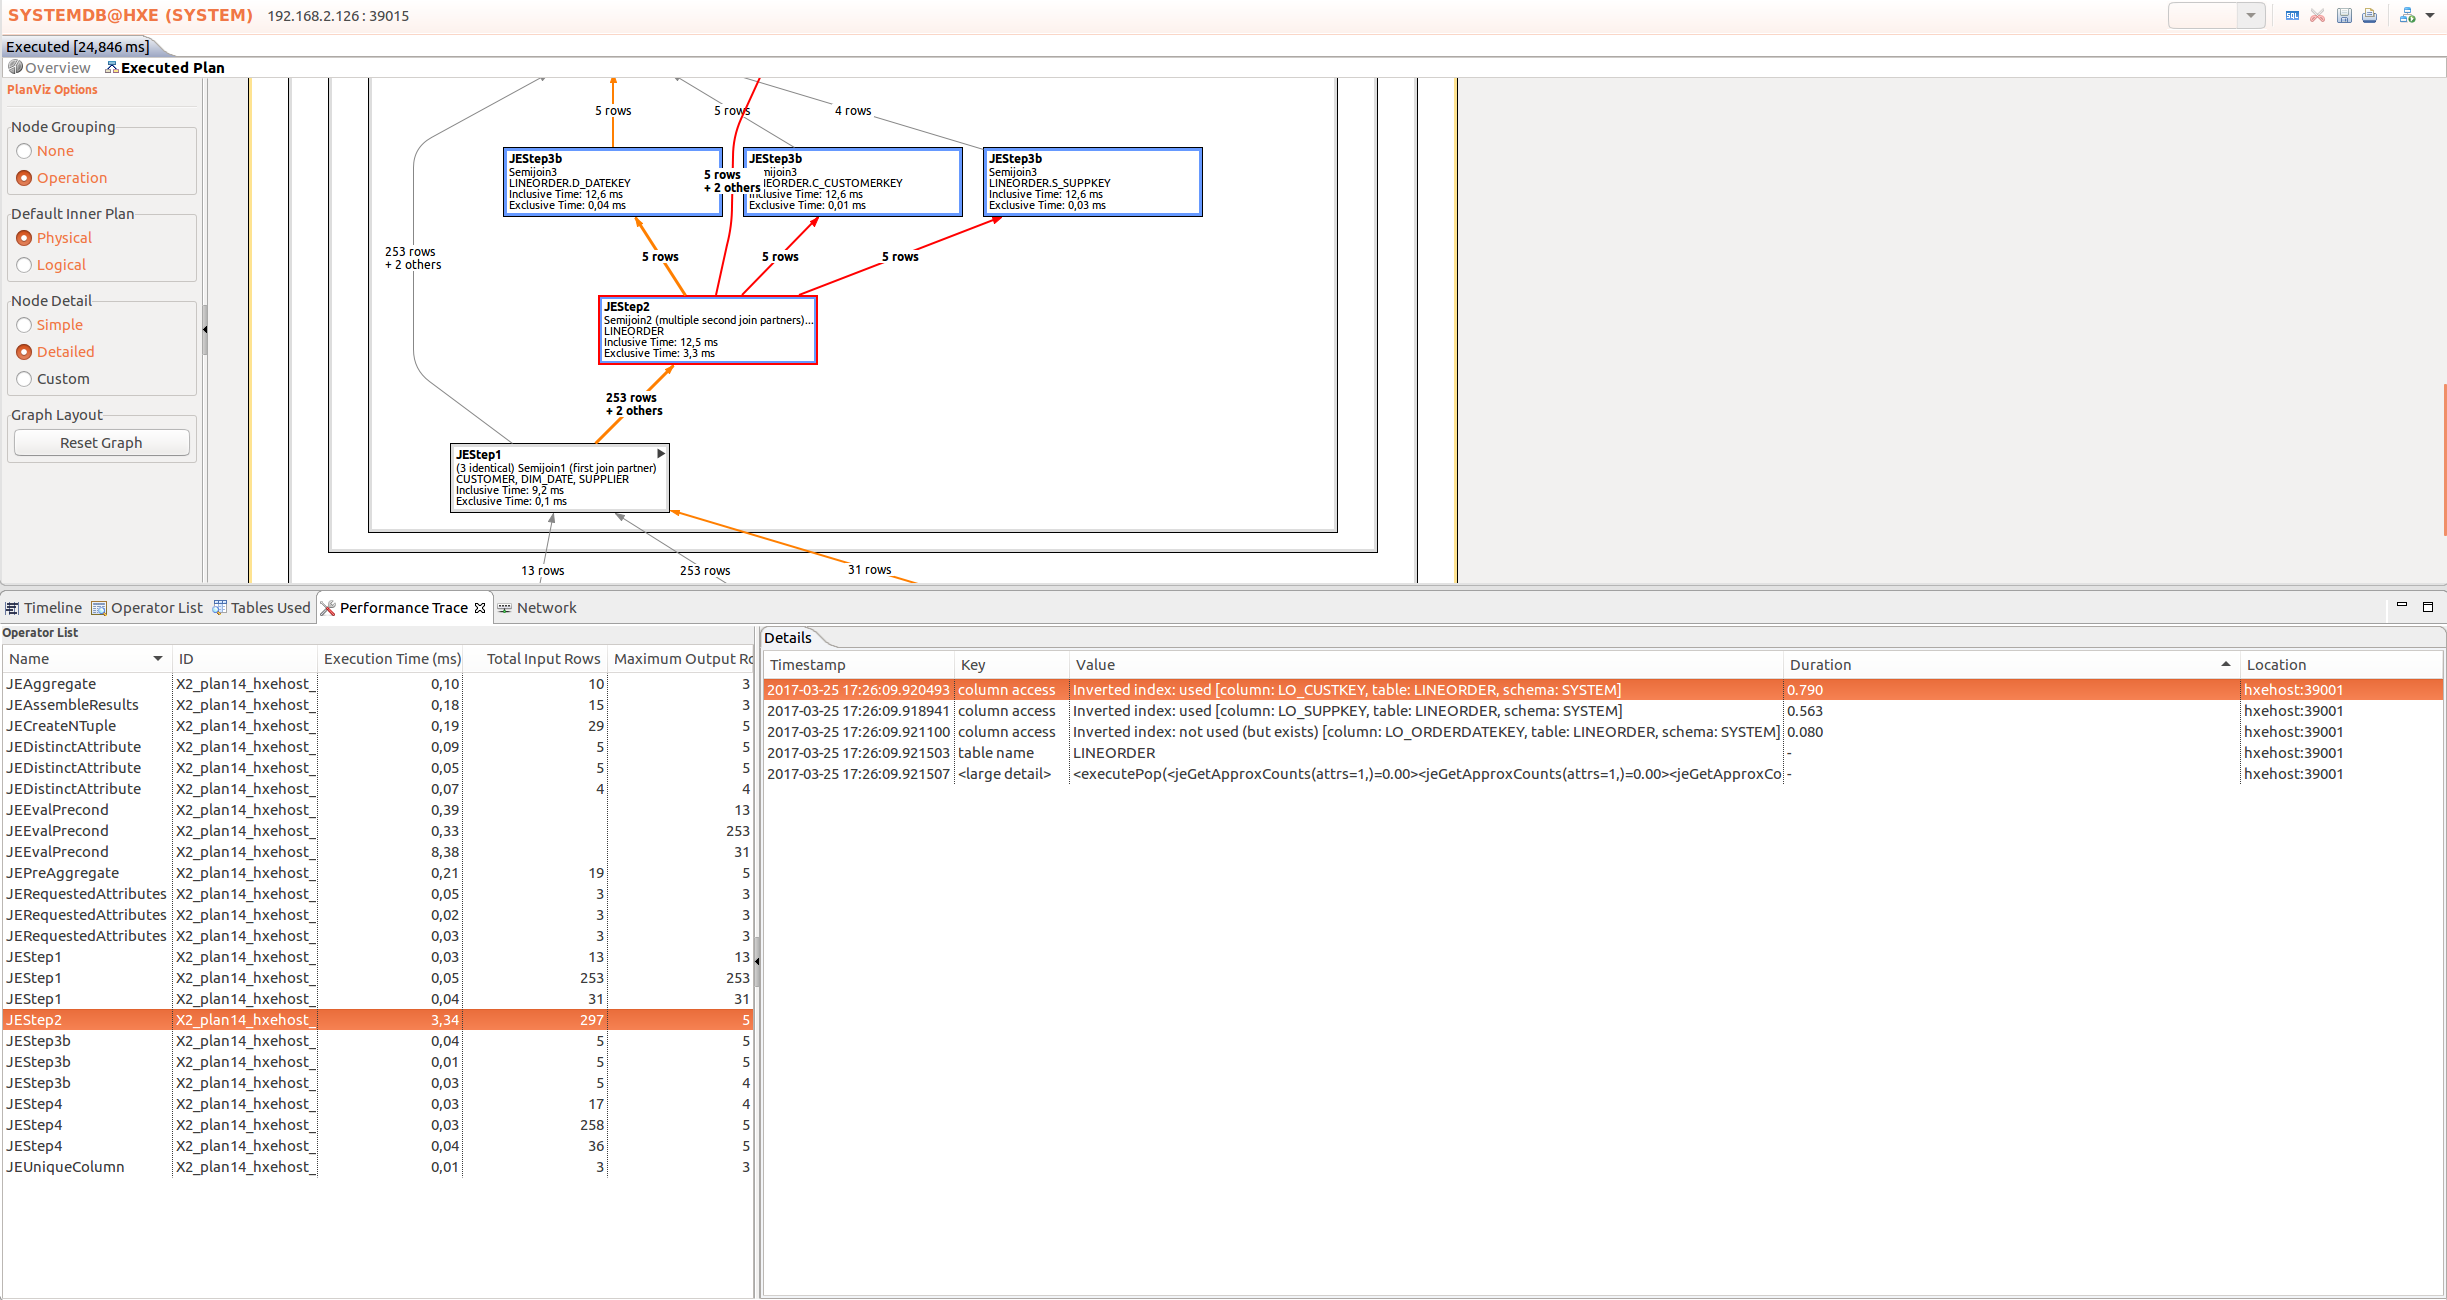
\includegraphics[scale=0.28]{images/execColIndex.png}
		\caption{Execution Plan: Q3.4 with Index}\label{execution-plan:after-index}
	\end{figure}
\end{landscape}
